
	\documentclass[letter]{article}
	\usepackage{amsmath,amssymb}
	\usepackage{enumitem}
	\usepackage{blindtext}
	\usepackage{booktabs}
	\usepackage{graphicx}
	
	\begin{document}
	
	\title{STAT 542 Homework 1}
	\author{Yifan Zhu}
	\maketitle
	
	\begin{enumerate}[leftmargin = 0 em, label = \arabic*., font = \bfseries]
	\item Approximately one-third of all human twins are identical (one-egg) and two-thirds are fraternal (two-egg) twins. Identical twins are necessarily the same sex, with male and female being equally likely. Among fraternal twins, approximately one-fourth are both female, one-fourth are both male, and half are one male and one female. Finally, among all U.S. births, approximately 1 in 90 is a twin birth. Define the following events:
	\begin{align*}
	&A = \{\textrm{a U.S. birth results in twin females}\}\\
	&B = \{\textrm{a U.S. birth results in identical twins}\}\\
	&C = \{\textrm{a U.S. birth results in twins}\}
	\end{align*}
	Find $P(A \cap B \cap C)$.

	$P(A\cap B \cap C) = P(A| B \cap C)P(B \cap C) = P(A | B \cap C)P(B | C) P(C) = \frac{1}{2} \frac{1}{3} \frac{1}{90} = \frac{1}{540}$

	\item Two litters of a particular rodent species have been born, one with two brown-haired and one gray-haired (litter 1), and the other with three brown-haired and two grayhaired (litter 2). We select a litter at random and then select an offspring at random from the selected litter.
	\begin{enumerate}[label = (\alph*), leftmargin = 0em]
		\item What is the probability that the animal chosen is brown-haired?

		$P(\{\textrm{brown-haired}\}) = P(\{\textrm{brown-haired}\} | \{\textrm{litter 1}\}) P(\{\textrm{litter 1}\}) 
		+\\ P(\{\textrm{brown-haired}\}| \{\textrm{litter 2}\}) P(\{\textrm{litter 2}\}) = \frac{2}{3} \cdot \frac{1}{2} + \frac{3}{5}\cdot \frac{1}{2} = \frac{19}{30}$
		\item Given that a brown-haired offspring was selected, what is the probability that the sampling was from litter 1?

		$P(\{\textrm{litter 1}\} | \{ \textrm{brown-haired}\}) = \frac{P(\{\textrm{brown-haired}\}\cap \{\textrm{litter 1}\})}{P(\{\textrm{brown-haired}\})} = \frac{P(\{\textrm{brown-haired}\}|\{\textrm{litter 1}\}) P(\{litter 1\})}{P(\{\textrm{brown-haired}\})} = \frac{2/3 \cdot 1/2}{19/30} = \frac{10}{19}$
	\end{enumerate}
	
	\item Prove each of the following statements. (Assume that any conditioning event has positive probability.)
	\begin{enumerate}[leftmargin = 0em]
		\item If $P(B) = 1$, then $P(A|B) = P(A)$ for any $A$.

		$P(A|B) = \frac{P(A \cap B)}{P(B)} = P(A \cap B) $. Also, we have $P(A) = P(A \cap B) + P(A \cap B^c)$. $P(B^c) = 1 - P(B) = 0$, $A\cap B^c \subset B^c \Rightarrow P(A\cap B^c) \leq P(B^c) = 0$. Thus $P(A \cap B^c) = 0$ and $P(A) = P(A \cap B)$. Therefore $P(A|B) = P(A\cap B) = P(A)$.
		\item If $A \subset B$, then $P(B|A) = 1$ and $P(A|B) = P(A)/P(B)$ .

		$A \subset B \Rightarrow A\cap B = A$.

		$P(B|A) = \frac{P(B\cap A)}{P(A)} = \frac{P(A)}{P(A)} =1$.

		$P(A|B) = \frac{P(A\cap B)}{P(B)} = \frac{P(A)}{P(B)}$
		\item If $A$ and $B$ are mutually exclusive, then
		\[P(A| A\cup B) = \frac{P(A)}{P(A)+P(B)}\]

		$A\subset A\cup B \Rightarrow A\cap (A\cup B) = A$, $A\cap B = \emptyset \Rightarrow P(A\cup B) = P(A) +P(B)$.

		$P(A|A\cup B) = \frac{A\cap (A\cup B)}{P(A\cup B)} = \frac{P(A)}{P(A)+P(B)}$

		\item $P(A\cap B\cap C) = P(A|B\cap C)P(B|C)P(C)$

		$P(A\cap B\cap C) = P(A\cap (B\cap C)) = P(A|B\cap C)P(B\cap C) = P(A|B\cap C)P(B|C)P(C)$
	\end{enumerate}
	
	\item A pair of events $A$ and $B$ cannot be simultaneously \emph{mutually exclusive} and \emph{independent}. Prove that if $P(A) > 0$ and $P(B) > 0$, then:
	\begin{enumerate}[leftmargin = 0em]
		\item If $A$ and $B$ are mutually exclusive, they cannot be independent.

		$A\cap B = \emptyset \Rightarrow P(A\cap B) = 0$. Therefore, $P(A|B) = \frac{P(A\cap B)}{P(B)} = 0 \neq P(A)$, as $P(A) >0$. Thus $A$ and $B$ are not independent.
		\item If $A$ and $B$ are independent, they cannot be mutually exclusive.

		$P(A|B) = P(A) \Rightarrow P(A\cap B) = P(A)P(B) >0$. Thus $A\cap B$ cannot be an empty set, $A$ and $B$ are not mutually exclusive.
	\end{enumerate}
	
	\item As in Example 1.3.6, consider telegraph signals ``dot''and ``dash'' sent in the proportion 3:4, where erratic transmissions cause a dot to become a dash with probability $\frac{1}{4}$ and a dash to become a dot with probability $\frac{1}{3}$.
	\begin{enumerate}[leftmargin = 0em]
		\item If a dash is received, what is the probability that a dash has been sent?

		$P(\{\textrm{dash sent}\}|\{\textrm{dash received}\}) = \frac{P(\{\textrm{dash sent}\}\cap \{\textrm{dash received}\})}{P(\{\textrm{dash received}\})}$.

		$P(\{\textrm{dash received}\}) = P(\{\textrm{dash received} | \textrm{dash sent}\}) P(\{\textrm{dash sent}\})+ \\
		P(\{\textrm{dash received}|\textrm{dot sent}\})P(\{\textrm{dot sent}\}) = \frac{2}{3} \cdot \frac{4}{7} + \frac{1}{4} \cdot \frac{3}{7} = \frac{41}{84}$.

		$P(\{\textrm{dash sent}\}\cap \{\textrm{dash received}\}) = P(\{\textrm{dash received}\}|\{\textrm{dash sent}\})P(\{\textrm{dash sent}\}) = \frac{2}{3} \cdot \frac{4}{7} = \frac{8}{21}$. 

		Therefore, $P(\{\textrm{dash sent}\}|\{\textrm{dash received}\}) = \frac{8/21}{41/84} = \frac{32}{41}$.
		\item Assuming independence between signals, if the message dot-dot was received, what is the probability distribution of the four possible messages that could have been sent?

		$P(\{\textrm{dot received}\} \cap \{\textrm{dot sent}\}) = P(\{\textrm{dot received}\}|\{\textrm{dot sent}\})P(\{\textrm{dot sent}\}) = \frac{3}{4} \cdot \frac{3}{7} = \frac{9}{28}$.

		$P(\{\textrm{dot received}\}) = 1 - P(\{\textrm{dash received}\}) = \frac{43}{84}$. 

		Thus, $P(\{\textrm{dot sent}\}|\{\textrm{dot received}\}) = \frac{(9/28)}{43/84} = \frac{27}{43}$, $P(\{\textrm{dash sent}\}|\{\textrm{dot received}\}) = \frac{16}{43}$. By indepence, the distribution of four messages could have been sent is:
		\begin{center}
		\begin{tabular}{cc}
		\toprule
		Signal sent & Probability\\ 
		\midrule
		dot-dot & $(27/43)^2$ \\
		dot-dash & $(27/43)\cdot (16/43)$\\
		dash-dot & $(16/43)\cdot(27/43)$\\
		dash-dash & $(16/43)^2$\\ 
		\bottomrule
		\end{tabular}
		\end{center}
	\end{enumerate}
	
	\item Prove that the following functions are cdfs.
	\begin{enumerate}[leftmargin = 0em, start = 3]
		\item $\mathrm{e}^{-\mathrm{e}^{-x}},\, x\in (-\infty, \infty)$
		\[F(x) = \mathrm{e}^{\mathrm{-e}^{-x}},\, x\in (-\infty, \infty)\]

		 $F(x)$ is right continuous. 
		 $\lim_{x\to -\infty} F(x) = 0, \, \lim_{x\to \infty} F(x) = 1$. 
		 $F'(x) = \mathrm{e}^{-x} \mathrm{e}^{-\mathrm{e}^{-x}} >0$. Thus $F(x)$ is a cdf.
		\item $1 - \mathrm{e}^{-x},\, x\in (0, \infty)$
		\[F(x) = \begin{cases}
		0& x\in (-\infty, 0]\\
		1 - \mathrm{e}^{-x} & x\in (0, \infty)
		\end{cases}\]
		$\lim_{x\to 0^{+}} F(x) = F(0) = 0$, $F(x)$ is right continuous. $\lim_{x\to -\infty} F(x) =0,\, \lim_{x\to \infty} F(x) = 1$. $F'(x) = \mathrm{e}^{-x} >0$. Thus $F(x)$ is a cdf.
	\end{enumerate}
	
	\item An appliance store receives a shipment of 30 microwave ovens, 5 of which are (unknown to the manager) defective. The store manager selects 4 ovens at random, without replacement, and tests to see if they are defective. Let $X = \textrm{number of defectives found}$. Calculate the pmf and cdf of $X$ and plot the cdf.
	\begin{align*}
	&P(X = 0) = \frac{\binom{25}{4}}{\binom{30}{4}} = 0.4616\\
	&P(X = 1) = \frac{\binom{5}{1}\binom{25}{3}}{\binom{30}{4}} = 0.4196\\
	&P(X = 2) = \frac{\binom{5}{2}\binom{25}{2}}{\binom{30}{4}} =  0.1095\\
	&P(X = 3) = \frac{\binom{5}{3}\binom{25}{2}}{\binom{30}{4}} =  0.0091\\
	&P(X = 4) = \frac{\binom{5}{4}\binom{25}{1}}{\binom{30}{4}} = 0.0002
	\end{align*}

	$F(x)$ is the cdf corresponding to the pmf above.
	\[F(x) = \begin{cases}
	0&x\in (-\infty, 0)\\
	0.4616 & x\in [0,1)\\
	0.8812 & x\in [1,2)\\
	0.9907 & x\in [2.3)\\
	0.9998 & x\in [3.4)\\
	1 & x\in [4,\infty)
	\end{cases}\]
	\begin{center}
	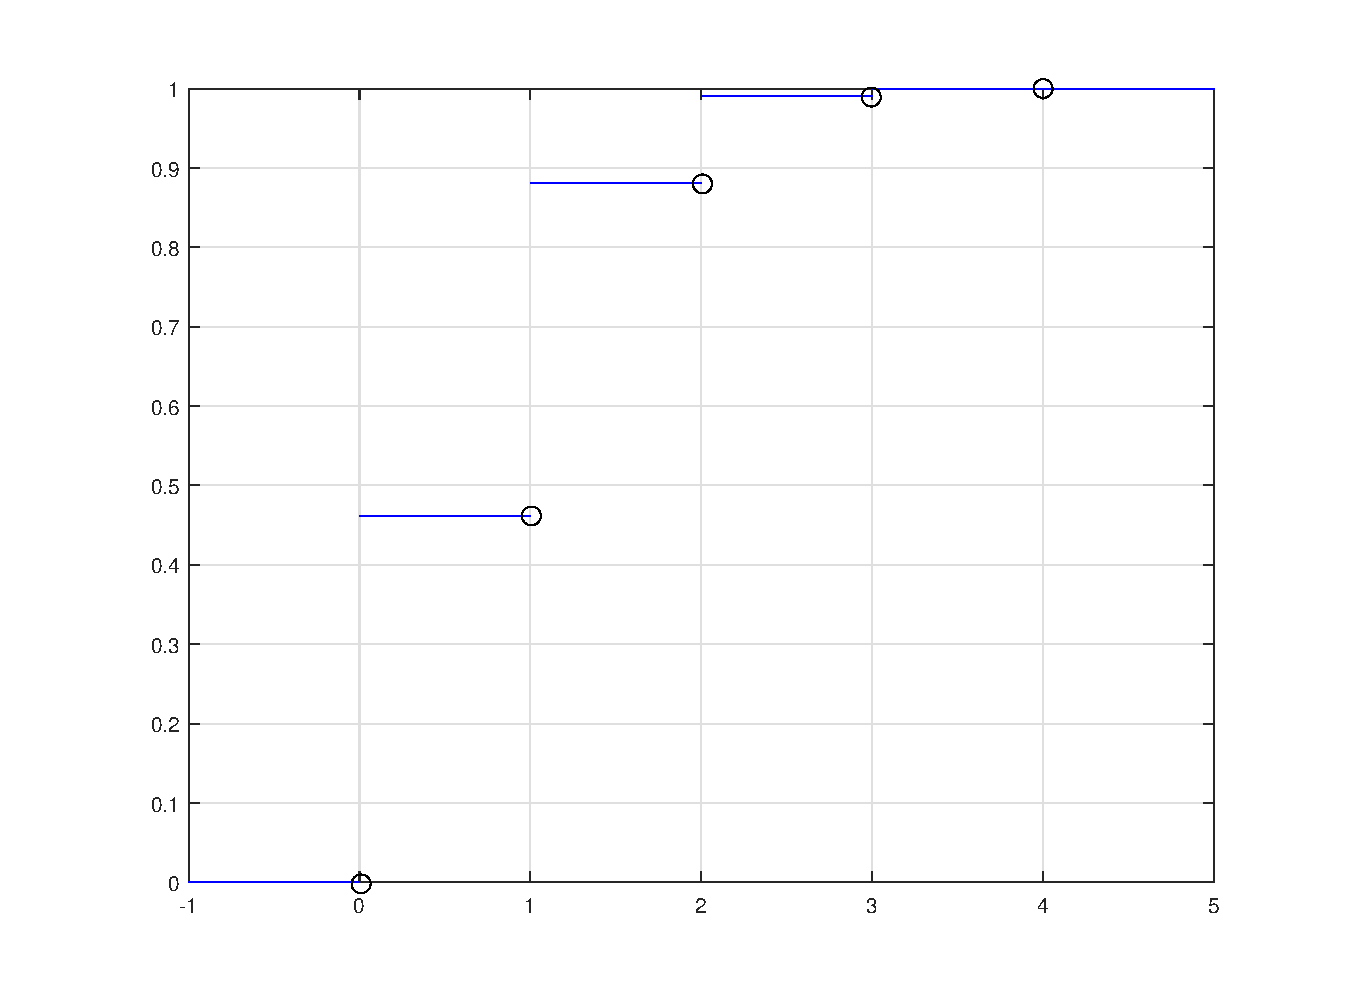
\includegraphics[width = 0.7\textwidth]{untitled.eps}
	\end{center}

	$P(3<X\leq 4.7) = P(X = 4) = 0.0002,\, P(3\leq X < 4.7) = P(X = 3) + P(X = 4) = 0.0093$.

	\item For each o f the following, determine the value of $c$ that makes $f(x)$ a pdf.
	\begin{enumerate}[leftmargin = 0em]
		\item $f(x) = c \sin(x) \mathrm{d}x,\, 0 < x < \pi/2$

		$\int_{0}^{\pi/2} c \sin x = c = 1 \Rightarrow c=1$.
		\item $f(x) = c \mathrm{e}^{-|x|},\, -\infty < x < \infty$

		$\int_{-\infty}^{\infty} c \mathrm{e}^{-|x|} \mathrm{d}x = 2c\int_{0}^{\infty} \mathrm{e}^{-x} = 2c =1 \Rightarrow c = 1/2$.
	\end{enumerate}
	
	\item From the axioms of probability, it follows that probability functions $P(\cdot)$ exhibit ``monotone continuity from above (mcfa)'', meaning that for any decreasing sequence of sets/events $A_1 \supset A_2 \supset A_3 \supset \cdots$,
	\[\lim_{n\to \infty} P(A_n) = P\left(\bigcap_{i = 1}^\infty A_i\right).\]
	Using the mcfa property, show that the cdf $F$ of a random variable $X$ must be right continuous: for any $x\in \mathbb{R}$, 
	\[\lim_{n\to \infty} F(x + n^{-1}) = F(x)\]
	holds.

	$F(x) = P_{X} (X \in (-\infty, x])$. Let $A_n = (-\infty, x + \frac{1}{n}]$, thus $A_1 \supset A_2 \supset A_3 \supset \cdots$, $\bigcap_{i=1}^{\infty} A_i = (-\infty, x]$.

	By mcfa, we have $\lim_{n\to \infty}F(x+n^{-1}) = \lim_{n\to\infty} P_{X}(A_n) = P_{X}(\bigcap_{i=1}^{\infty}A_i) = P_X ((-\infty, x]) = F(x)$.

	\item Statistical reliability involves studying the time to failure of manufactured units. In many reliability textbooks. one can find the exponential distribution
	\[f(x) = \begin{cases}
	\frac{1}{\theta} \mathrm{e}^{- x/\theta}&x>0\\
	0&x\leq 0
	\end{cases}\]
	where $\theta>0$ is a fixed value, for modeling the time $X$ that a random unit runs until failure (i.e. $X$ is a survival time). While a useful distribution gernerlly, the exponential distribution is not typically realistic for modeling failure times. Show that if $X$ has an exponential distribution as above, then 
	\[P(X > s+t|X>t) = P(X>s)\]
	for any calues $t,s >0$; this feature is called teh ``memoryless'' property of the exponential distribution. Explain intuitively why the ``memoryless'' property might make the exponential distribution an unappealing model for the survival time of a randomly selected, manufactured unit.

	$P(X > t ) = 1 - P(X\leq t) = 1 - F(t) = 1 - \int_{-\infty}^{t}f(x) \mathrm{d}x = 1 - \int_{0}^t f(x) \mathrm{d}x = 1 - (1 - \mathrm{e}^{-t/\theta}) = \mathrm{e}^{-t/\theta} $.

	Therefore, $P(X> s+t | X>t) = \frac{P(X\in (s+t, \infty)\cap (t, \infty))}{P(X>t)} = \frac{P(X>s+t)}{P(X>t)} = \frac{\mathrm{e}^{-(s+t)/\theta}}{\mathrm{e}^{-t/\theta}} = \mathrm{e}^{-s/\theta} = P(X>s)$

	The chance to survive a period of time $s$ for the manufactured unit should go down as the time the manufactured unit has already survived get longer, so the ``memoryless'' property of exponential distribution makes it an unappealing model.
 	\end{enumerate}


	
	
	
	\end{document}